%----------------------------------------------------------------------------------------
% PACKAGES AND OTHER DOCUMENT CONFIGURATIONS
%----------------------------------------------------------------------------------------
\documentclass{article}
\usepackage{fancyhdr} % Required for custom headers
\usepackage{lastpage} % Required to determine the last page for the footer
\usepackage{extramarks} % Required for headers and footers
\usepackage[usenames,dvipsnames]{color} % Required for custom colors
\usepackage{graphicx} % Required to insert images
\usepackage{listings} % Required for insertion of code
\usepackage{courier} % Required for the courier font
\usepackage{lipsum} % Used for inserting dummy 'Lorem ipsum' text into the template
\usepackage[utf8]{inputenc}
\usepackage[ngerman]{babel}
% Margins
\topmargin=-0.45in
\evensidemargin=0in
\oddsidemargin=0in
\textwidth=6.5in
\textheight=9.0in
\headsep=0.25in
\linespread{1.1} % Line spacing
% Set up the header and footer
\pagestyle{fancy}
%\lhead{\hmwkAuthorName} % Top left header
\chead{\hmwkClass\ : \hmwkTitle} % Top center head
\rhead{\firstxmark} % Top right header
\lfoot{\lastxmark} % Bottom left footer
\cfoot{} % Bottom center footer
\rfoot{Page\ \thepage\ of\ \protect\pageref{LastPage}} % Bottom right footer
\renewcommand\headrulewidth{0.4pt} % Size of the header rule
\renewcommand\footrulewidth{0.4pt} % Size of the footer rule
\setlength\parindent{0pt} % Removes all indentation from paragraphs
%----------------------------------------------------------------------------------------
% CODE INCLUSION CONFIGURATION
%----------------------------------------------------------------------------------------
\definecolor{MyDarkGreen}{rgb}{0.0,0.4,0.0} % This is the color used for comments
\lstloadlanguages{Perl} % Load Perl syntax for listings, for a list of other languages supported see: ftp://ftp.tex.ac.uk/tex-archive/macros/latex/contrib/listings/listings.pdf
\lstset{language=Perl, % Use Perl in this example
frame=single, % Single frame around code
basicstyle=\small\ttfamily, % Use small true type font
keywordstyle=[1]\color{Blue}\bf, % Perl functions bold and blue
keywordstyle=[2]\color{Purple}, % Perl function arguments purple
keywordstyle=[3]\color{Blue}\underbar, % Custom functions underlined and blue
identifierstyle=, % Nothing special about identifiers
commentstyle=\usefont{T1}{pcr}{m}{sl}\color{MyDarkGreen}\small, % Comments small dark green courier font
stringstyle=\color{Purple}, % Strings are purple
showstringspaces=false, % Don't put marks in string spaces
tabsize=5, % 5 spaces per tab
%
% Put standard Perl functions not included in the default language here
morekeywords={rand},
%
% Put Perl function parameters here
morekeywords=[2]{on, off, interp},
%
% Put user defined functions here
morekeywords=[3]{test},
%
morecomment=[l][\color{Blue}]{...}, % Line continuation (...) like blue comment
numbers=left, % Line numbers on left
firstnumber=1, % Line numbers start with line 1
numberstyle=\tiny\color{Blue}, % Line numbers are blue and small
stepnumber=5 % Line numbers go in steps of 5
}
% Creates a new command to include a perl script, the first parameter is the filename of the script (without .pl), the second parameter is the caption
\newcommand{\perlscript}[2]{
\begin{itemize}
\item[]\lstinputlisting[caption=#2,label=#1]{#1.pl}
\end{itemize}
}
%----------------------------------------------------------------------------------------
% DOCUMENT STRUCTURE COMMANDS
% Skip this unless you know what you're doing
%----------------------------------------------------------------------------------------
% Header and footer for when a page split occurs within a problem environment
\newcommand{\enterProblemHeader}[1]{
%\nobreak\extramarks{#1}{#1 continued on next page\ldots}\nobreak
%\nobreak\extramarks{#1 (continued)}{#1 continued on next page\ldots}\nobreak
}
% Header and footer for when a page split occurs between problem environments
\newcommand{\exitProblemHeader}[1]{
%\nobreak\extramarks{#1 (continued)}{#1 continued on next page\ldots}\nobreak
%\nobreak\extramarks{#1}{}\nobreak
}
\setcounter{secnumdepth}{0} % Removes default section numbers
\newcounter{homeworkProblemCounter} % Creates a counter to keep track of the number of problems
\newcommand{\homeworkProblemName}{}
\newenvironment{homeworkProblem}[1][Problem \arabic{homeworkProblemCounter}]{ % Makes a new environment called homeworkProblem which takes 1 argument (custom name) but the default is "Problem #"
\stepcounter{homeworkProblemCounter} % Increase counter for number of problems
\renewcommand{\homeworkProblemName}{#1} % Assign \homeworkProblemName the name of the problem
\section{\homeworkProblemName} % Make a section in the document with the custom problem count
%\enterProblemHeader{\homeworkProblemName} % Header and footer within the environment
}{
%\exitProblemHeader{\homeworkProblemName} % Header and footer after the environment
}
\newcommand{\problemAnswer}[1]{ % Defines the problem answer command with the content as the only argument
\noindent\framebox[\columnwidth][c]{\begin{minipage}{0.98\columnwidth}#1\end{minipage}} % Makes the box around the problem answer and puts the content inside
}
\newcommand{\homeworkSectionName}{}
\newenvironment{homeworkSection}[1]{ % New environment for sections within homework problems, takes 1 argument - the name of the section
\renewcommand{\homeworkSectionName}{#1} % Assign \homeworkSectionName to the name of the section from the environment argument
\subsection{\homeworkSectionName} % Make a subsection with the custom name of the subsection
%\enterProblemHeader{\homeworkProblemName\ [\homeworkSectionName]} % Header and footer within the environment
}{
%\enterProblemHeader{\homeworkProblemName} % Header and footer after the environment
}
%----------------------------------------------------------------------------------------
% NAME AND CLASS SECTION
%----------------------------------------------------------------------------------------
\newcommand{\hmwkTitle}{Übung\ \#8} % Assignment title
\newcommand{\hmwkDueDate}{Mittwoch,\ 14.\ Januar\ 2015} % Due date
\newcommand{\hmwkClass}{Parallel Computer Architecture} % Course/class
\newcommand{\hmwkClassTime}{} % Class/lecture time
\newcommand{\hmwkClassInstructor}{} % Teacher/lecturer
\newcommand{\hmwkAuthorName}{Günther Schindler, Fabian Finkeldey, Shamna Shyju} % Your name
%----------------------------------------------------------------------------------------
% TITLE PAGE
%----------------------------------------------------------------------------------------
\title{
\vspace{2in}
\textmd{\textbf{\hmwkClass:\ \hmwkTitle}}\\
\normalsize\vspace{0.1in}\small{Abgabe\ am\ \hmwkDueDate}\\
\vspace{0.1in}\large{\textit{\hmwkClassTime}}
\vspace{3in}
}
\author{\textbf{\hmwkAuthorName}}
\date{} % Insert date here if you want it to appear below your name
%----------------------------------------------------------------------------------------
\begin{document}
\maketitle
%----------------------------------------------------------------------------------------
% TABLE OF CONTENTS
%----------------------------------------------------------------------------------------
%\setcounter{tocdepth}{1} % Uncomment this line if you don't want subsections listed in the ToC
\newpage
\tableofcontents
\newpage
%----------------------------------------------------------------------------------------
% Auswertung - N-Body Simulation revisited
%----------------------------------------------------------------------------------------
\begin{homeworkProblem}[Auswertung - N-Body Simulation revisited]
Im Zuge des achten Übungszettels, ist die bereits realisierte N-Body-Parallelisierung,
via OpenMP auszuwerten. Es soll für verschieden Problemgrößen (128 - 8192 Bodies) die
Threadanzahl (2 - 16) variiert und die Ausführungszeit sowie der Speed-Up ermittelt
werden. Die Ergebnisse sind tabellarisch festzuhalten.
\\\\
Nachfolgende Tabelle zeigt nun die Ergebnisse der Ausführungszeiten der N-Body
Berechnung. 

\begin{center}
\begin{tabular}{|c|c|c|c|c|c|c|c|}\hline
   Threads & \multicolumn{7}{c|}{Ausführungszeit [ms]} \\ \hline
      & 128   & 256   & 512   & 1024 & 2048 & 4096 & 8192 \\ \hline
    2 & 0.150 & 0.519 & 2.444 & 8.269 & 36.137 & 135.521 & 495.916 \\ \hline
    4 & 0.084 & 0.282 & 1.189 & 4.527 & 16.457 & 58.126 & 258.995 \\ \hline
    6 & 0.055 & 0.181 & 0.804 & 3.001 & 10.676 & 43.652 & 176.471 \\ \hline
    8 & 0.045 & 0.152 & 0.652 & 2.567 & 8.574 & 34.839 & 148.560 \\ \hline
    12 & 0.033 & 0.100 & 0.460 & 1.699 & 6.282 & 23.424 & 81.303 \\ \hline
    16 & 0.026 & 0.088 & 0.333 & 1.1142 & 4.646 & 17.365 & 63.650 \\ \hline
 \end{tabular}
\end{center}
Visualisiert man diese Ergebnisse und trägt logarithmisch die Ausführungszeiten in 
Abhängigkeit von der Threadanzahl auf, verdeutlicht sich das Ergebniss. Wie erwartet
steigen die Ausführungszeiten exponentiell mit Verdoppelung der Problemgröße. Auch
sinken die Ausführungszeiten mit Erhöhung der Threadanzahl.
\begin{center}
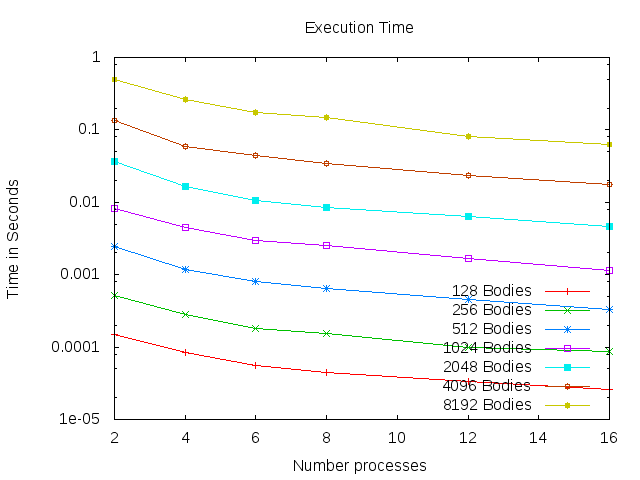
\includegraphics[width=0.7\columnwidth]{exec-time}
\end{center}
Weiter wurden auch der jeweilige Speed-Up ermittelt und wie folgt tabellarisch
festgehalten.
\begin{center}
\begin{tabular}{|c|c|c|c|c|c|c|c|}\hline
   Threads & \multicolumn{7}{c|}{Speed-Up} \\ \hline
      & 128   & 256   & 512   & 1024 & 2048 & 4096 & 8192 \\ \hline
    2 & 1.90 & 1.62 & 0.92 & 1.07 & 0.98 & 1.05 & 1.14 \\ \hline
    4 & 3.47 & 2.97 & 1.86 & 1.97 & 2.16 & 2.44 & 2.19 \\ \hline
    6 & 5.52 & 4.63 & 2.76 & 2.97 & 3.33 & 3.25 & 3.20 \\ \hline
    8 & 6.58 & 5.50 & 3.52 & 3.45 & 4.13 & 4.06 & 3.81 \\ \hline
    12 & 8.89 & 8.35 & 4.98 & 5.25 & 5.64 & 6.06 & 6.96 \\ \hline
    16 & 11.26 & 9.47 & 7.02 & 7.76 & 7.63 & 8.15 & 8.86 \\ \hline
 \end{tabular}
\end{center}
Für eine bessere Interpretation wurden auch diese Resultate visualisiert. 
\begin{center}
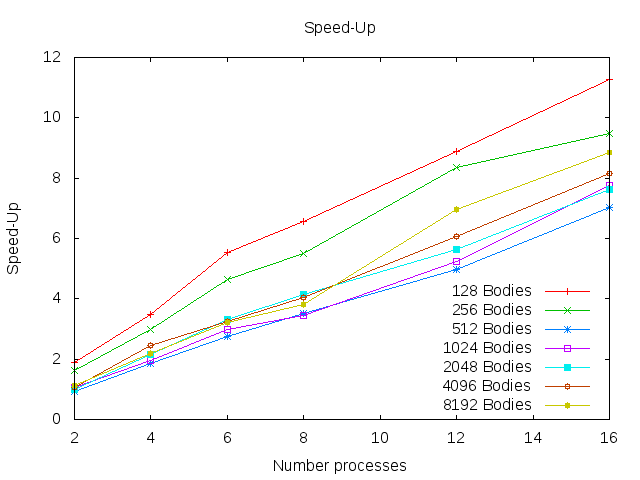
\includegraphics[width=0.7\columnwidth]{speed-up}
\end{center}
Auffällig hierbei ist, dass sich der Speed-Up der Problemgrößen 128 und 256 deutlich
von den anderen Problegrößen abhebt, wobei der Speed-Up bei 128 Bodies am größten ist.
Betrachtet man die größe eines Bodies könnte die effektive Nutzung des L1 Caches der
Grund hierfür sein. 
\end{homeworkProblem}

%----------------------------------------------------------------------------------------
% Hello World! - MPI
%----------------------------------------------------------------------------------------
%\begin{homeworkProblem}[Hello World! - MPI]

%\begin{lstlisting}{c}
%\end{lstlisting}

%\begin{center}
%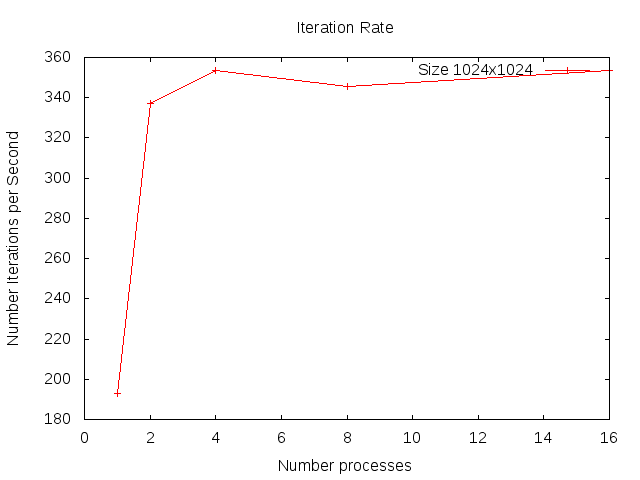
\includegraphics[width=0.7\columnwidth]{iteration-rate}
%\end{center}

%\end{homeworkProblem}

%----------------------------------------------------------------------------------------
% Half-round-trip latency - MPI
%----------------------------------------------------------------------------------------
\begin{homeworkProblem}[Half-round-trip latency - MPI]
Als nächstes ist die Half-round-trip latency mit MPI innerhalbe eines Knotens, 
bzw. zwischen zwei Knoten zu messen. Dies soll für Nachrichtengrößen zwischen $2^0$
- $2^{20}$ mit Gigabit Ethernet passieren.

\begin{center}
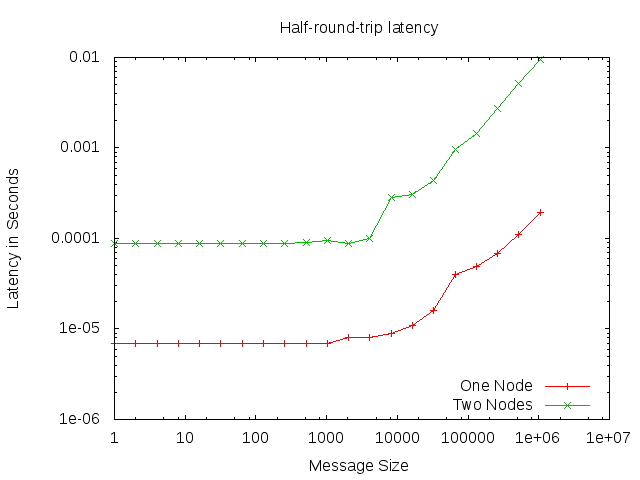
\includegraphics[width=0.7\columnwidth]{round-trip}
\end{center}

Die Latenzzeiten sind wie erwartet auf einem Knoten viel schneller als zwischen zwei
Knoten. Es fällt auf, dass die Latenzzeiten ab einer Nachrichtengrößen von 8 kByte
stark ansteigen. Dies könnte an der Maximum Transmission Unit (MTU) von Gigabit 
Ethernet liegen. Da hier die MTU auf 9 kByte beschränkt ist muss je 9 kByte Nachrichtenblock
ein zusätzlicher Frame gesendet werden.
\end{homeworkProblem}
\pagebreak

\end{document}
